% Options for packages loaded elsewhere
\PassOptionsToPackage{unicode}{hyperref}
\PassOptionsToPackage{hyphens}{url}
\documentclass[
]{article}
\usepackage{xcolor}
\usepackage[margin=1in]{geometry}
\usepackage{amsmath,amssymb}
\setcounter{secnumdepth}{5}
\usepackage{iftex}
\ifPDFTeX
  \usepackage[T1]{fontenc}
  \usepackage[utf8]{inputenc}
  \usepackage{textcomp} % provide euro and other symbols
\else % if luatex or xetex
  \usepackage{unicode-math} % this also loads fontspec
  \defaultfontfeatures{Scale=MatchLowercase}
  \defaultfontfeatures[\rmfamily]{Ligatures=TeX,Scale=1}
\fi
\usepackage{lmodern}
\ifPDFTeX\else
  % xetex/luatex font selection
\fi
% Use upquote if available, for straight quotes in verbatim environments
\IfFileExists{upquote.sty}{\usepackage{upquote}}{}
\IfFileExists{microtype.sty}{% use microtype if available
  \usepackage[]{microtype}
  \UseMicrotypeSet[protrusion]{basicmath} % disable protrusion for tt fonts
}{}
\makeatletter
\@ifundefined{KOMAClassName}{% if non-KOMA class
  \IfFileExists{parskip.sty}{%
    \usepackage{parskip}
  }{% else
    \setlength{\parindent}{0pt}
    \setlength{\parskip}{6pt plus 2pt minus 1pt}}
}{% if KOMA class
  \KOMAoptions{parskip=half}}
\makeatother
\usepackage{color}
\usepackage{fancyvrb}
\newcommand{\VerbBar}{|}
\newcommand{\VERB}{\Verb[commandchars=\\\{\}]}
\DefineVerbatimEnvironment{Highlighting}{Verbatim}{commandchars=\\\{\}}
% Add ',fontsize=\small' for more characters per line
\usepackage{framed}
\definecolor{shadecolor}{RGB}{248,248,248}
\newenvironment{Shaded}{\begin{snugshade}}{\end{snugshade}}
\newcommand{\AlertTok}[1]{\textcolor[rgb]{0.94,0.16,0.16}{#1}}
\newcommand{\AnnotationTok}[1]{\textcolor[rgb]{0.56,0.35,0.01}{\textbf{\textit{#1}}}}
\newcommand{\AttributeTok}[1]{\textcolor[rgb]{0.13,0.29,0.53}{#1}}
\newcommand{\BaseNTok}[1]{\textcolor[rgb]{0.00,0.00,0.81}{#1}}
\newcommand{\BuiltInTok}[1]{#1}
\newcommand{\CharTok}[1]{\textcolor[rgb]{0.31,0.60,0.02}{#1}}
\newcommand{\CommentTok}[1]{\textcolor[rgb]{0.56,0.35,0.01}{\textit{#1}}}
\newcommand{\CommentVarTok}[1]{\textcolor[rgb]{0.56,0.35,0.01}{\textbf{\textit{#1}}}}
\newcommand{\ConstantTok}[1]{\textcolor[rgb]{0.56,0.35,0.01}{#1}}
\newcommand{\ControlFlowTok}[1]{\textcolor[rgb]{0.13,0.29,0.53}{\textbf{#1}}}
\newcommand{\DataTypeTok}[1]{\textcolor[rgb]{0.13,0.29,0.53}{#1}}
\newcommand{\DecValTok}[1]{\textcolor[rgb]{0.00,0.00,0.81}{#1}}
\newcommand{\DocumentationTok}[1]{\textcolor[rgb]{0.56,0.35,0.01}{\textbf{\textit{#1}}}}
\newcommand{\ErrorTok}[1]{\textcolor[rgb]{0.64,0.00,0.00}{\textbf{#1}}}
\newcommand{\ExtensionTok}[1]{#1}
\newcommand{\FloatTok}[1]{\textcolor[rgb]{0.00,0.00,0.81}{#1}}
\newcommand{\FunctionTok}[1]{\textcolor[rgb]{0.13,0.29,0.53}{\textbf{#1}}}
\newcommand{\ImportTok}[1]{#1}
\newcommand{\InformationTok}[1]{\textcolor[rgb]{0.56,0.35,0.01}{\textbf{\textit{#1}}}}
\newcommand{\KeywordTok}[1]{\textcolor[rgb]{0.13,0.29,0.53}{\textbf{#1}}}
\newcommand{\NormalTok}[1]{#1}
\newcommand{\OperatorTok}[1]{\textcolor[rgb]{0.81,0.36,0.00}{\textbf{#1}}}
\newcommand{\OtherTok}[1]{\textcolor[rgb]{0.56,0.35,0.01}{#1}}
\newcommand{\PreprocessorTok}[1]{\textcolor[rgb]{0.56,0.35,0.01}{\textit{#1}}}
\newcommand{\RegionMarkerTok}[1]{#1}
\newcommand{\SpecialCharTok}[1]{\textcolor[rgb]{0.81,0.36,0.00}{\textbf{#1}}}
\newcommand{\SpecialStringTok}[1]{\textcolor[rgb]{0.31,0.60,0.02}{#1}}
\newcommand{\StringTok}[1]{\textcolor[rgb]{0.31,0.60,0.02}{#1}}
\newcommand{\VariableTok}[1]{\textcolor[rgb]{0.00,0.00,0.00}{#1}}
\newcommand{\VerbatimStringTok}[1]{\textcolor[rgb]{0.31,0.60,0.02}{#1}}
\newcommand{\WarningTok}[1]{\textcolor[rgb]{0.56,0.35,0.01}{\textbf{\textit{#1}}}}
\usepackage{graphicx}
\makeatletter
\newsavebox\pandoc@box
\newcommand*\pandocbounded[1]{% scales image to fit in text height/width
  \sbox\pandoc@box{#1}%
  \Gscale@div\@tempa{\textheight}{\dimexpr\ht\pandoc@box+\dp\pandoc@box\relax}%
  \Gscale@div\@tempb{\linewidth}{\wd\pandoc@box}%
  \ifdim\@tempb\p@<\@tempa\p@\let\@tempa\@tempb\fi% select the smaller of both
  \ifdim\@tempa\p@<\p@\scalebox{\@tempa}{\usebox\pandoc@box}%
  \else\usebox{\pandoc@box}%
  \fi%
}
% Set default figure placement to htbp
\def\fps@figure{htbp}
\makeatother
\setlength{\emergencystretch}{3em} % prevent overfull lines
\providecommand{\tightlist}{%
  \setlength{\itemsep}{0pt}\setlength{\parskip}{0pt}}
\usepackage{fontspec}
\setmainfont{Libertinus Serif}
\usepackage{bookmark}
\IfFileExists{xurl.sty}{\usepackage{xurl}}{} % add URL line breaks if available
\urlstyle{same}
\hypersetup{
  pdftitle={p-demotion-discourse},
  pdfauthor={Cristian R. Juárez},
  hidelinks,
  pdfcreator={LaTeX via pandoc}}

\title{p-demotion-discourse}
\author{Cristian R. Juárez}
\date{2026-03-19}

\begin{document}
\maketitle

\begin{Shaded}
\begin{Highlighting}[]
\FunctionTok{library}\NormalTok{(tidyverse)}
\end{Highlighting}
\end{Shaded}

\begin{verbatim}
## -- Attaching core tidyverse packages ------------------------ tidyverse 2.0.0 --
## v dplyr     1.1.4     v readr     2.1.5
## v forcats   1.0.0     v stringr   1.5.1
## v ggplot2   3.5.1     v tibble    3.2.1
## v lubridate 1.9.3     v tidyr     1.3.1
## v purrr     1.0.2     
## -- Conflicts ------------------------------------------ tidyverse_conflicts() --
## x dplyr::filter() masks stats::filter()
## x dplyr::lag()    masks stats::lag()
## i Use the conflicted package (<http://conflicted.r-lib.org/>) to force all conflicts to become errors
\end{verbatim}

\begin{Shaded}
\begin{Highlighting}[]
\FunctionTok{library}\NormalTok{(viridis)}
\end{Highlighting}
\end{Shaded}

\begin{verbatim}
## Loading required package: viridisLite
\end{verbatim}

\begin{Shaded}
\begin{Highlighting}[]
\FunctionTok{library}\NormalTok{(viridisLite)}
\end{Highlighting}
\end{Shaded}

\begin{itemize}
\tightlist
\item
  Load data and first exploration
\end{itemize}

\begin{Shaded}
\begin{Highlighting}[]
\NormalTok{mocCA190924 }\OtherTok{\textless{}{-}} \FunctionTok{read.delim}\NormalTok{(}\StringTok{"/Users/cristian/Documents/postdocs/research/abst\_pprs\_docmnt/2025{-}pdemot{-}moc/raw\_data/mocCA190924\_text.tsv"}\NormalTok{, }\AttributeTok{sep =} \StringTok{"}\SpecialCharTok{\textbackslash{}t}\StringTok{"}\NormalTok{, }\AttributeTok{header =}\NormalTok{ T)}
\CommentTok{\# glimpse(mocCA190924)}
\CommentTok{\# head(mocCA190924)}
\end{Highlighting}
\end{Shaded}

\begin{itemize}
\tightlist
\item
  Distribution of predicate types (ok)
\end{itemize}

\begin{Shaded}
\begin{Highlighting}[]
\NormalTok{mocCA190924 }\SpecialCharTok{|\textgreater{}} 
  \FunctionTok{filter}\NormalTok{(}\SpecialCharTok{!}\FunctionTok{is.na}\NormalTok{(val\_type), val\_type }\SpecialCharTok{!=} \StringTok{""}\NormalTok{, val\_type }\SpecialCharTok{!=} \StringTok{"avalent"}\NormalTok{ ) }\SpecialCharTok{|\textgreater{}}
  \FunctionTok{arrange}\NormalTok{(val\_type) }\SpecialCharTok{|\textgreater{}} 
   \FunctionTok{count}\NormalTok{(val\_type) }\SpecialCharTok{|\textgreater{}} 
    \FunctionTok{arrange}\NormalTok{(}\FunctionTok{desc}\NormalTok{(n)) }\SpecialCharTok{|\textgreater{}}
  \FunctionTok{mutate}\NormalTok{(}\AttributeTok{proportion =}\NormalTok{ n }\SpecialCharTok{/} \FunctionTok{sum}\NormalTok{(n)) }\SpecialCharTok{|\textgreater{}}
  \FunctionTok{arrange}\NormalTok{(proportion) }\SpecialCharTok{|\textgreater{}}
\FunctionTok{ggplot}\NormalTok{(}\FunctionTok{aes}\NormalTok{(}\AttributeTok{x =} \FunctionTok{reorder}\NormalTok{( val\_type, proportion), }\AttributeTok{y =}\NormalTok{ proportion, }\AttributeTok{fill =}\NormalTok{ proportion)) }\SpecialCharTok{+}
  \FunctionTok{geom\_bar}\NormalTok{(}\AttributeTok{stat =} \StringTok{"identity"}\NormalTok{) }\SpecialCharTok{+}
\CommentTok{\# Add counts and proportion in bars  }
\FunctionTok{geom\_text}\NormalTok{(}\FunctionTok{aes}\NormalTok{(}\AttributeTok{label =} \FunctionTok{paste0}\NormalTok{(n, }\StringTok{"("}\NormalTok{, scales}\SpecialCharTok{::}\FunctionTok{percent}\NormalTok{(proportion), }\StringTok{")"}\NormalTok{)), }
            \AttributeTok{vjust =} \SpecialCharTok{{-}}\FloatTok{0.4}\NormalTok{,}
            \AttributeTok{size  =} \FloatTok{2.3}\NormalTok{,}
            \AttributeTok{color =} \StringTok{"black"}\NormalTok{) }\SpecialCharTok{+}
   \FunctionTok{scale\_fill\_viridis\_c}\NormalTok{(}\AttributeTok{option =} \StringTok{"D"}\NormalTok{) }\SpecialCharTok{+}
  
\CommentTok{\# If you prefer percentage ticks, use this instead:}
  \FunctionTok{scale\_y\_continuous}\NormalTok{(}\AttributeTok{limits =} \FunctionTok{c}\NormalTok{(}\DecValTok{0}\NormalTok{, }\FloatTok{0.5}\NormalTok{), }\AttributeTok{labels =}\NormalTok{ scales}\SpecialCharTok{::}\NormalTok{percent) }\SpecialCharTok{+}
  \FunctionTok{scale\_y\_continuous}\NormalTok{(}\AttributeTok{limits =} \FunctionTok{c}\NormalTok{(}\DecValTok{0}\NormalTok{, }\FloatTok{0.5}\NormalTok{)) }\SpecialCharTok{+}
  \CommentTok{\#scale\_fill\_gradient(low = "gray90", high = "gray10") +}
  \FunctionTok{labs}\NormalTok{(}\AttributeTok{title =} \StringTok{""}\NormalTok{,}
       \AttributeTok{x =} \StringTok{"Predicate type"}\NormalTok{,}
       \AttributeTok{y =} \StringTok{"Proportion"}\NormalTok{) }\SpecialCharTok{+}
  \FunctionTok{theme\_minimal}\NormalTok{() }\SpecialCharTok{+}
  \FunctionTok{theme}\NormalTok{( }
\CommentTok{\# Panel (plotting area) background}
    \AttributeTok{panel.background =} \FunctionTok{element\_rect}\NormalTok{(}\AttributeTok{fill =} \StringTok{"\#F2F2F2"}\NormalTok{, }\AttributeTok{colour =} \ConstantTok{NA}\NormalTok{),}
    \CommentTok{\# Add a subtle border around the panel (optional)}
    \AttributeTok{panel.border =} \FunctionTok{element\_rect}\NormalTok{(}\AttributeTok{fill =} \ConstantTok{NA}\NormalTok{, }\AttributeTok{colour =} \StringTok{"\#BDBDBD"}\NormalTok{, }\AttributeTok{size =} \FloatTok{0.5}\NormalTok{),}
  \AttributeTok{panel.grid.major =} \FunctionTok{element\_blank}\NormalTok{(),}
  \AttributeTok{panel.grid.minor =} \FunctionTok{element\_blank}\NormalTok{(),}
\CommentTok{\# Outer background (outside plotting area)}
    \AttributeTok{plot.background  =} \FunctionTok{element\_rect}\NormalTok{(}\AttributeTok{fill =} \StringTok{"white"}\NormalTok{, }\AttributeTok{colour =} \ConstantTok{NA}\NormalTok{),}
    \AttributeTok{legend.position =} \StringTok{"none"}\NormalTok{, }\AttributeTok{axis.text.x =} \FunctionTok{element\_text}\NormalTok{(}\AttributeTok{angle =} \DecValTok{45}\NormalTok{, }\AttributeTok{hjust =} \DecValTok{1}\NormalTok{),}
\AttributeTok{axis.title.x =} \FunctionTok{element\_text}\NormalTok{(}\AttributeTok{margin =} \FunctionTok{margin}\NormalTok{(}\AttributeTok{t =} \DecValTok{9}\NormalTok{, }\AttributeTok{r =} \DecValTok{5}\NormalTok{, }\AttributeTok{b =} \DecValTok{0}\NormalTok{, }\AttributeTok{l =} \DecValTok{0}\NormalTok{)),}
\AttributeTok{axis.title.y =} \FunctionTok{element\_text}\NormalTok{(}\AttributeTok{margin =} \FunctionTok{margin}\NormalTok{(}\AttributeTok{t =} \DecValTok{9}\NormalTok{, }\AttributeTok{r =} \DecValTok{9}\NormalTok{, }\AttributeTok{b =} \DecValTok{0}\NormalTok{, }\AttributeTok{l =} \DecValTok{0}\NormalTok{)), }
\NormalTok{)  }\CommentTok{\# Tilt labels 45 degrees)}
\end{Highlighting}
\end{Shaded}

\begin{verbatim}
## Scale for y is already present.
## Adding another scale for y, which will replace the existing scale.
\end{verbatim}

\begin{verbatim}
## Warning: The `size` argument of `element_rect()` is deprecated as of ggplot2 3.4.0.
## i Please use the `linewidth` argument instead.
## This warning is displayed once every 8 hours.
## Call `lifecycle::last_lifecycle_warnings()` to see where this warning was
## generated.
\end{verbatim}

\pandocbounded{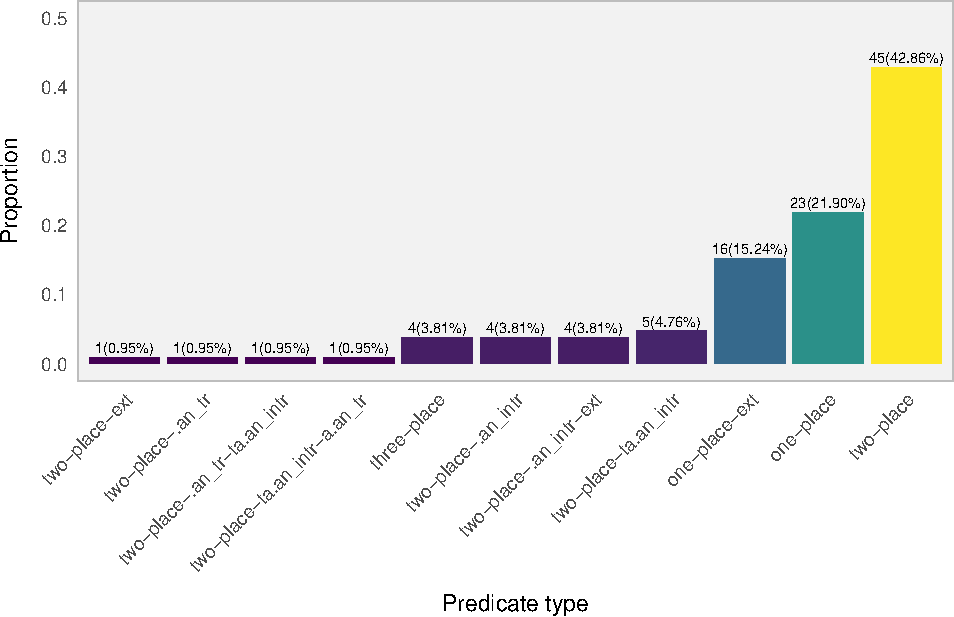
\includegraphics[keepaspectratio]{p-demotion_files/figure-latex/unnamed-chunk-3-1.pdf}}

\begin{Shaded}
\begin{Highlighting}[]
\CommentTok{\# Save plot in project\textquotesingle{}s folder}
\FunctionTok{ggsave}\NormalTok{(}\AttributeTok{filename =} \StringTok{"/Users/cristian/Documents/postdocs/research/abst\_pprs\_docmnt/2025{-}pdemot{-}moc/figures/proportion{-}predicates.png"}\NormalTok{,}
  \AttributeTok{plot =} \FunctionTok{last\_plot}\NormalTok{(),}
  \AttributeTok{width =} \DecValTok{7}\NormalTok{, }\AttributeTok{height =} \DecValTok{4}\NormalTok{,}
  \AttributeTok{dpi =} \DecValTok{600}\NormalTok{,          }\CommentTok{\# minimum for print}
\NormalTok{)}
\end{Highlighting}
\end{Shaded}

\begin{itemize}
\tightlist
\item
  Correspondence of predicates in -ɢan or -taɢan alternations. (ok)
\end{itemize}

\begin{Shaded}
\begin{Highlighting}[]
 \CommentTok{\# Table: distribution of predicates in text}
\NormalTok{ predicates }\OtherTok{\textless{}{-}}\NormalTok{ mocCA190924 }\SpecialCharTok{|\textgreater{}} 
   \FunctionTok{rename}\NormalTok{(}\AttributeTok{predicate\_type =}\NormalTok{ val\_type) }\SpecialCharTok{|\textgreater{}}
   \FunctionTok{filter}\NormalTok{(}\SpecialCharTok{!}\FunctionTok{is.na}\NormalTok{(verb\_in\_sentence), verb\_in\_sentence }\SpecialCharTok{!=} \StringTok{""}\NormalTok{, }\FunctionTok{str\_detect}\NormalTok{(predicate\_type, }\StringTok{"{-}ɢan|{-}taɢan"}\NormalTok{)) }\SpecialCharTok{|\textgreater{}}  \CommentTok{\# simplified search with regular expression. Better option}
   \FunctionTok{count}\NormalTok{(verb\_in\_sentence, predicate\_type) }\SpecialCharTok{|\textgreater{}} 
   \FunctionTok{arrange}\NormalTok{(}\FunctionTok{desc}\NormalTok{(n))}
\NormalTok{ predicates}
\end{Highlighting}
\end{Shaded}

\begin{verbatim}
##      verb_in_sentence               predicate_type n
## 1               speak       two-place-ɢan_intr-ext 4
## 2                know         two-place-taɢan_intr 3
## 3                work           two-place-ɢan_intr 2
## 4  ask_for_permission           two-place-ɢan_intr 1
## 5                 eat             two-place-ɢan_tr 1
## 6                 eat  two-place-ɢan_tr-taɢan_intr 1
## 7                know two-place-taɢan_intr-aɢan_tr 1
## 8            remember         two-place-taɢan_intr 1
## 9               speak           two-place-ɢan_intr 1
## 10 transfer_knowledge         two-place-taɢan_intr 1
\end{verbatim}

\begin{Shaded}
\begin{Highlighting}[]
 \CommentTok{\# Create table for document}
\FunctionTok{library}\NormalTok{(xtable) }
\NormalTok{predicates\_derived }\OtherTok{\textless{}{-}} \FunctionTok{xtable}\NormalTok{(predicates,}
             \AttributeTok{caption =} \StringTok{"Predicates by valency subtype"}\NormalTok{,}
             \AttributeTok{label   =} \StringTok{"tab:predicates"}\NormalTok{)}
\FunctionTok{print}\NormalTok{(predicates\_derived)}
\end{Highlighting}
\end{Shaded}

\begin{verbatim}
## % latex table generated in R 4.4.2 by xtable 1.8-4 package
## % Thu Mar 19 21:24:23 2026
## \begin{table}[ht]
## \centering
## \begin{tabular}{rllr}
##   \hline
##  & verb\_in\_sentence & predicate\_type & n \\ 
##   \hline
## 1 & speak & two-place-ɢan\_intr-ext &   4 \\ 
##   2 & know & two-place-taɢan\_intr &   3 \\ 
##   3 & work & two-place-ɢan\_intr &   2 \\ 
##   4 & ask\_for\_permission & two-place-ɢan\_intr &   1 \\ 
##   5 & eat & two-place-ɢan\_tr &   1 \\ 
##   6 & eat & two-place-ɢan\_tr-taɢan\_intr &   1 \\ 
##   7 & know & two-place-taɢan\_intr-aɢan\_tr &   1 \\ 
##   8 & remember & two-place-taɢan\_intr &   1 \\ 
##   9 & speak & two-place-ɢan\_intr &   1 \\ 
##   10 & transfer\_knowledge & two-place-taɢan\_intr &   1 \\ 
##    \hline
## \end{tabular}
## \caption{Predicates by valency subtype} 
## \label{tab:predicates}
## \end{table}
\end{verbatim}

\begin{itemize}
\tightlist
\item
  Observe correspondences between expression/abscence of P arguments
  (ok)
\end{itemize}

\begin{Shaded}
\begin{Highlighting}[]
\CommentTok{\# Table: val\_type vs P\_arg}
\NormalTok{p\_expression }\OtherTok{\textless{}{-}}\NormalTok{ mocCA190924 }\SpecialCharTok{|\textgreater{}} 
   \FunctionTok{rename}\NormalTok{(}\AttributeTok{predicate\_type =}\NormalTok{ val\_type) }\SpecialCharTok{|\textgreater{}} 
  \FunctionTok{filter}\NormalTok{(}\SpecialCharTok{!}\FunctionTok{is.na}\NormalTok{(predicate\_type), predicate\_type }\SpecialCharTok{!=} \StringTok{""}\NormalTok{, }\FunctionTok{str\_detect}\NormalTok{(predicate\_type, }\StringTok{"{-}ɢan|{-}taɢan"}\NormalTok{),}
         \SpecialCharTok{!}\FunctionTok{is.na}\NormalTok{(P\_arg), P\_arg }\SpecialCharTok{!=} \StringTok{""}\NormalTok{, P\_arg }\SpecialCharTok{!=} \StringTok{"not\_applicable"}\NormalTok{) }\SpecialCharTok{|\textgreater{}} 
  \FunctionTok{count}\NormalTok{(predicate\_type, P\_arg) }\SpecialCharTok{|\textgreater{}} 
  \FunctionTok{arrange}\NormalTok{(}\FunctionTok{desc}\NormalTok{(n)) }\SpecialCharTok{|\textgreater{}}
 \FunctionTok{mutate}\NormalTok{( }\AttributeTok{P\_arg =} \FunctionTok{recode}\NormalTok{(P\_arg,}
      \StringTok{"yes"}            \OtherTok{=} \StringTok{"P\_present"}\NormalTok{,}
     \StringTok{"no"}             \OtherTok{=} \StringTok{"P\_absent"}\NormalTok{)) }\SpecialCharTok{|\textgreater{}} 
  \FunctionTok{pivot\_wider}\NormalTok{(}\AttributeTok{names\_from =}\NormalTok{ P\_arg, }\AttributeTok{values\_from =}\NormalTok{ n, }\AttributeTok{values\_fill =} \DecValTok{0}\NormalTok{)}

\CommentTok{\# Check output }
\NormalTok{ p\_expression}
\end{Highlighting}
\end{Shaded}

\begin{verbatim}
## # A tibble: 6 x 3
##   predicate_type               P_present P_absent
##   <chr>                            <int>    <int>
## 1 two-place-ɢan_intr-ext               4        0
## 2 two-place-taɢan_intr                 2        3
## 3 two-place-ɢan_intr                   1        3
## 4 two-place-taɢan_intr-aɢan_tr         1        0
## 5 two-place-ɢan_tr                     1        0
## 6 two-place-ɢan_tr-taɢan_intr          0        1
\end{verbatim}

\begin{Shaded}
\begin{Highlighting}[]
\CommentTok{\# Create table for document}
\FunctionTok{library}\NormalTok{(xtable) }
\NormalTok{p\_expression\_tab }\OtherTok{\textless{}{-}} \FunctionTok{xtable}\NormalTok{(p\_expression,}
             \AttributeTok{caption =} \StringTok{"P expression"}\NormalTok{,}
             \AttributeTok{label   =} \StringTok{"tab:p\_expression"}\NormalTok{)}
\FunctionTok{print}\NormalTok{(p\_expression\_tab)}
\end{Highlighting}
\end{Shaded}

\begin{verbatim}
## % latex table generated in R 4.4.2 by xtable 1.8-4 package
## % Thu Mar 19 21:24:23 2026
## \begin{table}[ht]
## \centering
## \begin{tabular}{rlrr}
##   \hline
##  & predicate\_type & P\_present & P\_absent \\ 
##   \hline
## 1 & two-place-ɢan\_intr-ext &   4 &   0 \\ 
##   2 & two-place-taɢan\_intr &   2 &   3 \\ 
##   3 & two-place-ɢan\_intr &   1 &   3 \\ 
##   4 & two-place-taɢan\_intr-aɢan\_tr &   1 &   0 \\ 
##   5 & two-place-ɢan\_tr &   1 &   0 \\ 
##   6 & two-place-ɢan\_tr-taɢan\_intr &   0 &   1 \\ 
##    \hline
## \end{tabular}
## \caption{P expression} 
## \label{tab:p_expression}
## \end{table}
\end{verbatim}

\begin{itemize}
\tightlist
\item
  Additional data organization: Test for semantic map
\end{itemize}

\begin{Shaded}
\begin{Highlighting}[]
\FunctionTok{library}\NormalTok{(dplyr)}
\FunctionTok{library}\NormalTok{(stringr)}
\CommentTok{\# Optional plotting libs used later:}
\CommentTok{\# library(ggplot2); library(viridis); library(ggrepel)}

\CommentTok{\# Start from your data frame: mocCA190924}
\NormalTok{df\_sem }\OtherTok{\textless{}{-}}\NormalTok{ mocCA190924 }\SpecialCharTok{\%\textgreater{}\%}
  \FunctionTok{filter}\NormalTok{(}
    \SpecialCharTok{!}\FunctionTok{is.na}\NormalTok{(verb\_in\_sentence), verb\_in\_sentence }\SpecialCharTok{!=} \StringTok{""}\NormalTok{,}
    \SpecialCharTok{!}\FunctionTok{is.na}\NormalTok{(val\_type), val\_type }\SpecialCharTok{!=} \StringTok{""}\NormalTok{, val\_type }\SpecialCharTok{!=} \StringTok{"not\_applicable"}\NormalTok{,}
\NormalTok{    val\_type }\SpecialCharTok{!=} \StringTok{"avalent"}                       \CommentTok{\# you asked to drop this earlier}
\NormalTok{  )}

\CommentTok{\# Optional: focus on P{-}demotion{-}relevant tokens}
\CommentTok{\# df\_sem \textless{}{-} df\_sem \%\textgreater{}\% filter(P\_arg == "yes")   \# uncomment if you want this restriction}

\CommentTok{\# Optional: keep only valency types that occur \textgreater{}= 2 tokens (stability)}
\NormalTok{min\_n }\OtherTok{\textless{}{-}} \DecValTok{1}
\NormalTok{keep\_val }\OtherTok{\textless{}{-}}\NormalTok{ df\_sem }\SpecialCharTok{\%\textgreater{}\%} \FunctionTok{count}\NormalTok{(val\_type) }\SpecialCharTok{\%\textgreater{}\%} \FunctionTok{filter}\NormalTok{(n }\SpecialCharTok{\textgreater{}=}\NormalTok{ min\_n) }\SpecialCharTok{\%\textgreater{}\%} \FunctionTok{pull}\NormalTok{(val\_type)}
\NormalTok{df\_sem }\OtherTok{\textless{}{-}}\NormalTok{ df\_sem }\SpecialCharTok{\%\textgreater{}\%} \FunctionTok{filter}\NormalTok{(val\_type }\SpecialCharTok{\%in\%}\NormalTok{ keep\_val)}

\FunctionTok{library}\NormalTok{(tidyr)}
\FunctionTok{library}\NormalTok{(FactoMineR)}
\FunctionTok{library}\NormalTok{(factoextra)}
\end{Highlighting}
\end{Shaded}

\begin{verbatim}
## Welcome! Want to learn more? See two factoextra-related books at https://goo.gl/ve3WBa
\end{verbatim}

\begin{Shaded}
\begin{Highlighting}[]
\CommentTok{\# 1) Build contingency table: predicates × valency types}
\NormalTok{tab }\OtherTok{\textless{}{-}}\NormalTok{ df\_sem }\SpecialCharTok{\%\textgreater{}\%}
  \FunctionTok{count}\NormalTok{(verb\_in\_sentence, val\_type) }\SpecialCharTok{\%\textgreater{}\%}
  \FunctionTok{pivot\_wider}\NormalTok{(}\AttributeTok{names\_from =}\NormalTok{ val\_type, }\AttributeTok{values\_from =}\NormalTok{ n, }\AttributeTok{values\_fill =} \DecValTok{0}\NormalTok{) }\SpecialCharTok{\%\textgreater{}\%}
\NormalTok{  tibble}\SpecialCharTok{::}\FunctionTok{column\_to\_rownames}\NormalTok{(}\StringTok{"verb\_in\_sentence"}\NormalTok{)}
\NormalTok{tab}
\end{Highlighting}
\end{Shaded}

\begin{verbatim}
##                    two-place one-place one-place-ext two-place-ɢan_intr
## approach                   1         0             0                  0
## arrive                     0         2             1                  0
## ask_for_permission         2         0             0                  1
## attach                     0         0             1                  0
## augment                    0         1             0                  0
## be                         0         4             2                  0
## be_equal                   1         0             0                  0
## be_happy                   0         1             0                  0
## be_next_to                 0         0             3                  0
## be_similar                 0         1             0                  0
## can                        1         0             0                  0
## come                       0         0             1                  0
## come_back                  0         1             0                  0
## depart                     0         1             3                  0
## eat                        0         0             0                  0
## exist                      0         5             0                  0
## exist.neg                  0         2             0                  0
## fight                      1         0             0                  0
## find                       1         0             0                  0
## get.married                0         1             0                  0
## get_redy                   0         1             0                  0
## give                       0         0             0                  0
## go                         0         2             1                  0
## help                       2         0             0                  0
## hit                        1         0             0                  0
## hunt                       0         0             1                  0
## know                       7         0             0                  0
## let_free                   1         0             0                  0
## look                       1         0             0                  0
## look_for                   1         0             0                  0
## move                       0         0             1                  0
## move_feet                  0         1             0                  0
## receive                    1         0             0                  0
## remember                   3         0             0                  0
## say                        2         0             0                  0
## see                        5         0             0                  0
## speak                      0         0             0                  1
## take                       4         0             0                  0
## take_care                  2         0             0                  0
## talk                       0         0             2                  0
## transfer_knowledge         7         0             0                  0
## wake_up                    1         0             0                  0
## work                       0         0             0                  2
##                    two-place-ɢan_tr two-place-ɢan_tr-taɢan_intr three-place
## approach                          0                           0           0
## arrive                            0                           0           0
## ask_for_permission                0                           0           0
## attach                            0                           0           0
## augment                           0                           0           0
## be                                0                           0           0
## be_equal                          0                           0           0
## be_happy                          0                           0           0
## be_next_to                        0                           0           0
## be_similar                        0                           0           0
## can                               0                           0           0
## come                              0                           0           0
## come_back                         0                           0           0
## depart                            0                           0           0
## eat                               1                           1           0
## exist                             0                           0           0
## exist.neg                         0                           0           0
## fight                             0                           0           0
## find                              0                           0           0
## get.married                       0                           0           0
## get_redy                          0                           0           0
## give                              0                           0           4
## go                                0                           0           0
## help                              0                           0           0
## hit                               0                           0           0
## hunt                              0                           0           0
## know                              0                           0           0
## let_free                          0                           0           0
## look                              0                           0           0
## look_for                          0                           0           0
## move                              0                           0           0
## move_feet                         0                           0           0
## receive                           0                           0           0
## remember                          0                           0           0
## say                               0                           0           0
## see                               0                           0           0
## speak                             0                           0           0
## take                              0                           0           0
## take_care                         0                           0           0
## talk                              0                           0           0
## transfer_knowledge                0                           0           0
## wake_up                           0                           0           0
## work                              0                           0           0
##                    two-place-ext two-place-taɢan_intr
## approach                       0                    0
## arrive                         0                    0
## ask_for_permission             0                    0
## attach                         0                    0
## augment                        0                    0
## be                             0                    0
## be_equal                       0                    0
## be_happy                       0                    0
## be_next_to                     0                    0
## be_similar                     0                    0
## can                            0                    0
## come                           0                    0
## come_back                      0                    0
## depart                         0                    0
## eat                            0                    0
## exist                          0                    0
## exist.neg                      0                    0
## fight                          0                    0
## find                           0                    0
## get.married                    0                    0
## get_redy                       0                    0
## give                           1                    0
## go                             0                    0
## help                           0                    0
## hit                            0                    0
## hunt                           0                    0
## know                           0                    3
## let_free                       0                    0
## look                           0                    0
## look_for                       0                    0
## move                           0                    0
## move_feet                      0                    0
## receive                        0                    0
## remember                       0                    1
## say                            0                    0
## see                            0                    0
## speak                          0                    0
## take                           0                    0
## take_care                      0                    0
## talk                           0                    0
## transfer_knowledge             0                    1
## wake_up                        0                    0
## work                           0                    0
##                    two-place-taɢan_intr-aɢan_tr two-place-ɢan_intr-ext
## approach                                      0                      0
## arrive                                        0                      0
## ask_for_permission                            0                      0
## attach                                        0                      0
## augment                                       0                      0
## be                                            0                      0
## be_equal                                      0                      0
## be_happy                                      0                      0
## be_next_to                                    0                      0
## be_similar                                    0                      0
## can                                           0                      0
## come                                          0                      0
## come_back                                     0                      0
## depart                                        0                      0
## eat                                           0                      0
## exist                                         0                      0
## exist.neg                                     0                      0
## fight                                         0                      0
## find                                          0                      0
## get.married                                   0                      0
## get_redy                                      0                      0
## give                                          0                      0
## go                                            0                      0
## help                                          0                      0
## hit                                           0                      0
## hunt                                          0                      0
## know                                          1                      0
## let_free                                      0                      0
## look                                          0                      0
## look_for                                      0                      0
## move                                          0                      0
## move_feet                                     0                      0
## receive                                       0                      0
## remember                                      0                      0
## say                                           0                      0
## see                                           0                      0
## speak                                         0                      4
## take                                          0                      0
## take_care                                     0                      0
## talk                                          0                      0
## transfer_knowledge                            0                      0
## wake_up                                       0                      0
## work                                          0                      0
\end{verbatim}

\begin{Shaded}
\begin{Highlighting}[]
\CommentTok{\# 2) Run CA}
\NormalTok{res.ca }\OtherTok{\textless{}{-}} \FunctionTok{CA}\NormalTok{(tab, }\AttributeTok{graph =} \ConstantTok{FALSE}\NormalTok{)}

\CommentTok{\# 3) Plot a clean biplot (semantic map)}
\FunctionTok{fviz\_ca\_biplot}\NormalTok{(}
\NormalTok{  res.ca,}
  \AttributeTok{repel =} \ConstantTok{TRUE}\NormalTok{,}
  \AttributeTok{col.row =} \StringTok{"\#2b2b2b"}\NormalTok{,   }\CommentTok{\# predicates}
  \AttributeTok{col.col =} \StringTok{"\#8c2d04"}\NormalTok{,   }\CommentTok{\# valency types}
  \AttributeTok{label =} \StringTok{"all"}\NormalTok{,}
  \AttributeTok{title =} \StringTok{"Predicate × Valency CA biplot (Mocoví)"}
\NormalTok{)}
\end{Highlighting}
\end{Shaded}

\pandocbounded{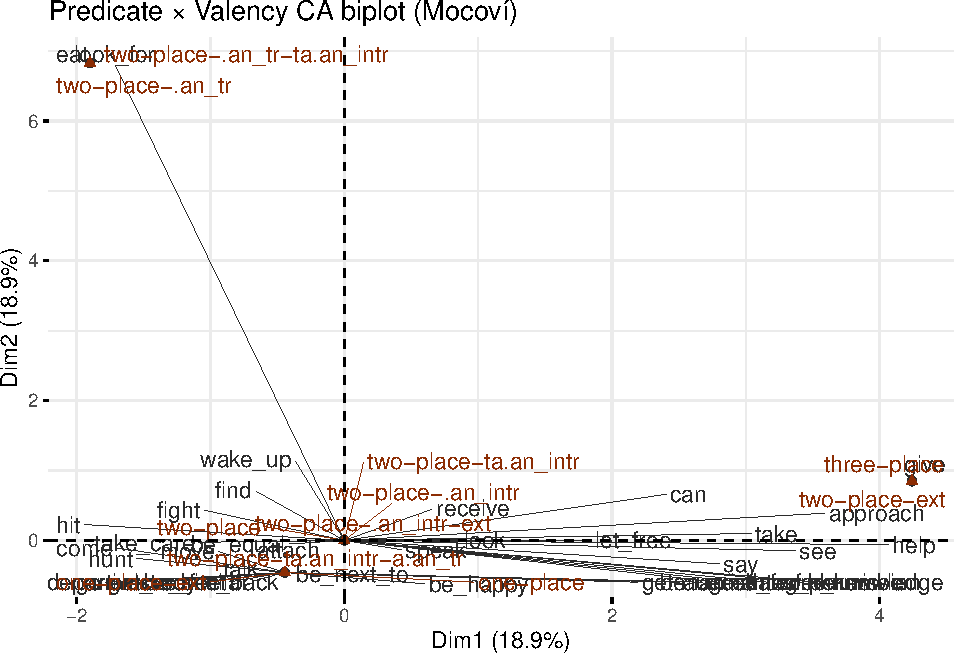
\includegraphics[keepaspectratio]{p-demotion_files/figure-latex/unnamed-chunk-6-1.pdf}}

\end{document}
